\documentclass[a4paper]{memoir}
\usepackage{graphicx}
%% Language and font encodings
\usepackage{microtype}
\usepackage[paperheight=88.9mm,paperwidth=63.5mm,margin=5mm]{geometry}
\usepackage{ragged2e}
\usepackage{adjustbox}
\usepackage{emoji}
\usepackage{pgffor}
\usepackage{tikz}
\newcommand{\cardtext}{1-12}
\newcommand{\grouptext}{2-6}
\newcommand{\agetext}{12+}
\newcommand{\clocktext}{25$''$}
\newcommand{\languagecrop}{french_crop}
\newcommand{\colorcount}{5}
\newcommand{\cardtitle}{}
\def\colors{0/myyellow, 1/myorange, 2/myred, 3/mypurple, 4/myblue}
\begin{document}
{\footnotesize
\setemojifont{NotoColorEmoji.ttf}[Path=../../../fonts/noto-emoji/]
\DeclareMicrotypeAlias{NotoColorEmoji.ttf}{TU-basic}
\newlength{\boxwidth}
\setlength{\boxwidth}{6.1mm}
\newlength{\boxheight}
\setlength{\boxheight}{9.2mm}
\newlength{\boxx}
\setlength{\boxx}{3.9mm}
\newlength{\boxy}
\setlength{\boxy}{4.3mm}
\newlength{\boxspacex}
\setlength{\boxspacex}{.4mm}
\newlength{\boxspacey}
\setlength{\boxspacey}{.4mm}
\newlength{\coldotspace}
\setlength{\coldotspace}{3.5mm}

% Define custom colors
\definecolor{myyellow}{rgb}{0.961, 0.745, 0.0}    
\definecolor{myblue}{rgb}{0.0, 0.439, 0.753}      
\definecolor{mygreen}{rgb}{0.039, 0.827, 0.376}   
\definecolor{myred}{rgb}{0.961, 0.0, 0.0}         
\definecolor{mypurple}{rgb}{0.718, 0.039, 0.718}  
\definecolor{myorange}{rgb}{1.0, 0.471, 0.039}  
\definecolor{myLighterGrey}{rgb}{0.9, 0.9, 0.9}

\begin{tikzpicture}[remember picture, overlay]
    \node[yshift=-14mm] (logo) at (current page.north)
    {
\includegraphics[width=\textwidth]{logo_alpha.png}};

    \node[yshift=1.4mm] (title) at (logo.south)
    {\cardtitle};

    \node[yshift=1.5mm, anchor=west] (qr) at (logo.west)
    {
\includegraphics[width=.267\textwidth]{qr-code.png}};

    \node[yshift=-1mm] (language) at (qr.south)
    {\adjustbox{width=.083\textwidth, height=.0498\textwidth, cfbox=black .4pt 0cm}{\includegraphics[width=.083\textwidth, height=.0498\textwidth]{../../../rule_lib/\languagecrop.png}}};

    \node[fill=myLighterGrey, xshift=-\boxx, yshift=\boxy, rounded corners, minimum width=\boxwidth, minimum height=\boxheight] (box1) at (logo.east) {};
    \node[fill=myLighterGrey, yshift=-\boxspacey-\boxheight/2, rounded corners, minimum width=\boxwidth, minimum height=\boxheight] (box2) at (box1.south) {};
    \node[fill=myLighterGrey, xshift=-\boxspacex-\boxwidth/2, rounded corners, minimum width=\boxwidth, minimum height=\boxheight] (box3) at (box1.west) {};
    \node[fill=myLighterGrey, yshift=-\boxspacey-\boxheight/2, rounded corners, minimum width=\boxwidth, minimum height=\boxheight] (box4) at (box3.south) {};

    \node[yshift=2.2mm] (cards) at (box1.center) {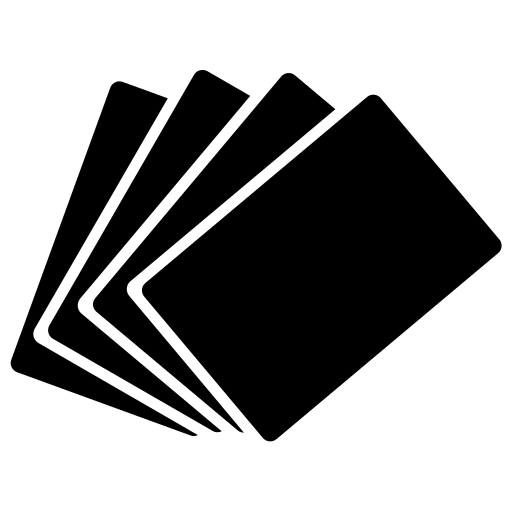
\includegraphics[width=.1\textwidth]{../../../rule_lib/cards.png}};
    \node (cards text) at (cards.south) {\cardtext};


    \foreach \i/\color in \colors {
        \ifnum \i<\colorcount
        \node[circle, fill=\color,  minimum size=3pt, scale=0.25,  xshift= (\i-.5*\colorcount+.5)*\coldotspace] (11) at (cards text.south){}; 
        \fi
    }

    \node[yshift=1.3mm] (group) at (box2.center) {
\includegraphics[width=.1\textwidth]{../../../rule_lib/group.png}};
    \node (group text) at (group.south) {\grouptext};

    \node[yshift=1.5mm] (age) at (box3.center) {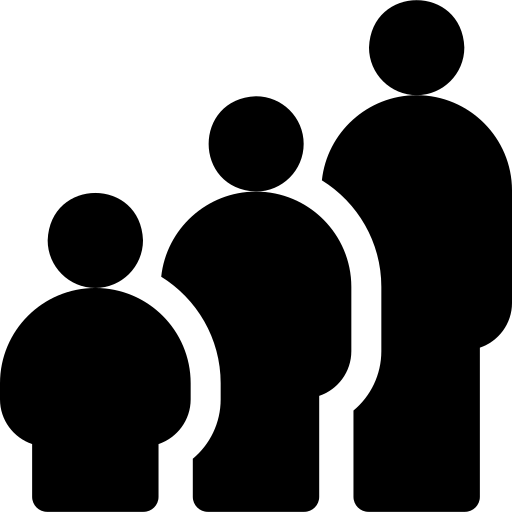
\includegraphics[width=.1\textwidth]{../../../rule_lib/age.png}};
    \node[yshift=-.5mm] (age text) at (age.south) {\agetext};

    \node[yshift=1.5mm] (clock) at (box4.center) {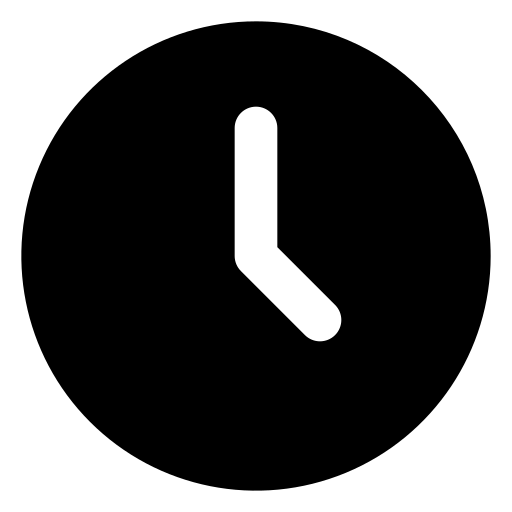
\includegraphics[width=.1\textwidth]{../../../rule_lib/clock.png}};
    \node[yshift=-.5mm] (clock text) at (clock.south) {\clocktext};
\end{tikzpicture}
\pagestyle{empty}
\justifying
$$ $$
\\
\\
\\
\\

\noindent
\textbf{\emoji{arrows-counterclockwise} Mise en place.} Mélange les cartes et donne en 4 cartes à chaque joueur. 
Le reste forme la pioche. Tu auras \textbf{des lignes de cartes} dans ta \textbf{zone} de jeu.
Les lignes du haut et du bas sont les lignes \textbf{actives}.
\\
\\
\textbf{\emoji{minus} Règles des lignes.} Elles ne sont créées \textbf{qu'en haut ou en bas}, 
doivent toujours rester de la \textbf{même couleur} et valent \textbf{leur carte la plus haute} en point.
% Le joueur avec le plus de points gagne, chaque ligne valant sa carte la plus haute.
\\
\\
\noindent
\textbf{\emoji{joystick} Déroulement.}  
Premier tour : pose une carte pour créer ta première ligne et pioche une carte. 
Tours suivants :
\begin{itemize}
    \item \emoji{warning} Tu \textbf{dois} jouer une carte dans la zone d’un adversaire pour créer ou incrémenter une \textbf{ligne active}.
    \item \emoji{seedling} Joue une autre carte dans ta zone pour incrémenter une ligne \textbf{(active ou non)} ou créer une nouvelle ligne
    (l'ancienne ligne active doit avoir une carte de même valeur, \textbf{un 10, 11, 12 ne peut pas être joué ainsi}). Tu peux ignorer cette étape en défaussant une carte. Termine ton tour en piochant 2 cartes.
\end{itemize} 
\textbf{\emoji{stop-sign} Fin de partie.}
Quand une zone a 4 lignes de couleurs différentes, le tour en cours se termine normalement et les autres joueurs jouent chacun \textbf{un dernier tour}.
\\
\\
\noindent
\emoji{pushpin} Tu peux avoir plusieurs lignes de la même couleur.
\\
\textbf{\emoji{pushpin} Lignes inactives.} Mets-les à côté de ta zone pour faire de la place, en ne conservant que la carte de valeur maximale pour chaque ligne (les autres sont défaussées).
}\end{document}